\subsection{Funzionamento di Kepler}

Kepler opera combinando due meccanismi complementari per associare i 
consumi energetici ai singoli container. Il primo è un programma eBPF 
(Extended Berkeley Packet Filter) integrato nel kernel, che traccia 
l'attività dei processi e li associa ai container tramite il file 
\texttt{/proc/PID/cgroup}, consentendo di correlare il Process ID di 
ciascun processo all'identificatore del container che lo ospita. Il 
secondo è l'interfaccia RAPL (Running Average Power Limit), disponibile 
sui processori Intel e AMD moderni, che permette di leggere i contatori 
energetici cumulativi direttamente dai registri hardware della CPU.

Una volta raccolti i dati di utilization dei processi e di consumo 
energetico del sistema, Kepler applica il \emph{Ratio Power Model} per 
attribuire a ciascun container la propria quota di consumo: la potenza 
dinamica viene distribuita tra i container in proporzione alla loro 
utilization rispetto all'utilization totale del sistema. Il risultato 
viene aggregato a livello di container e reso disponibile tramite 
Prometheus nella metrica \texttt{kepler\_container\_cpu\_joules\_total}, 
un contatore cumulativo espresso in Joule che cresce monotonicamente nel 
tempo per ogni container attivo.

\begin{figure}[ht]
    \centering
    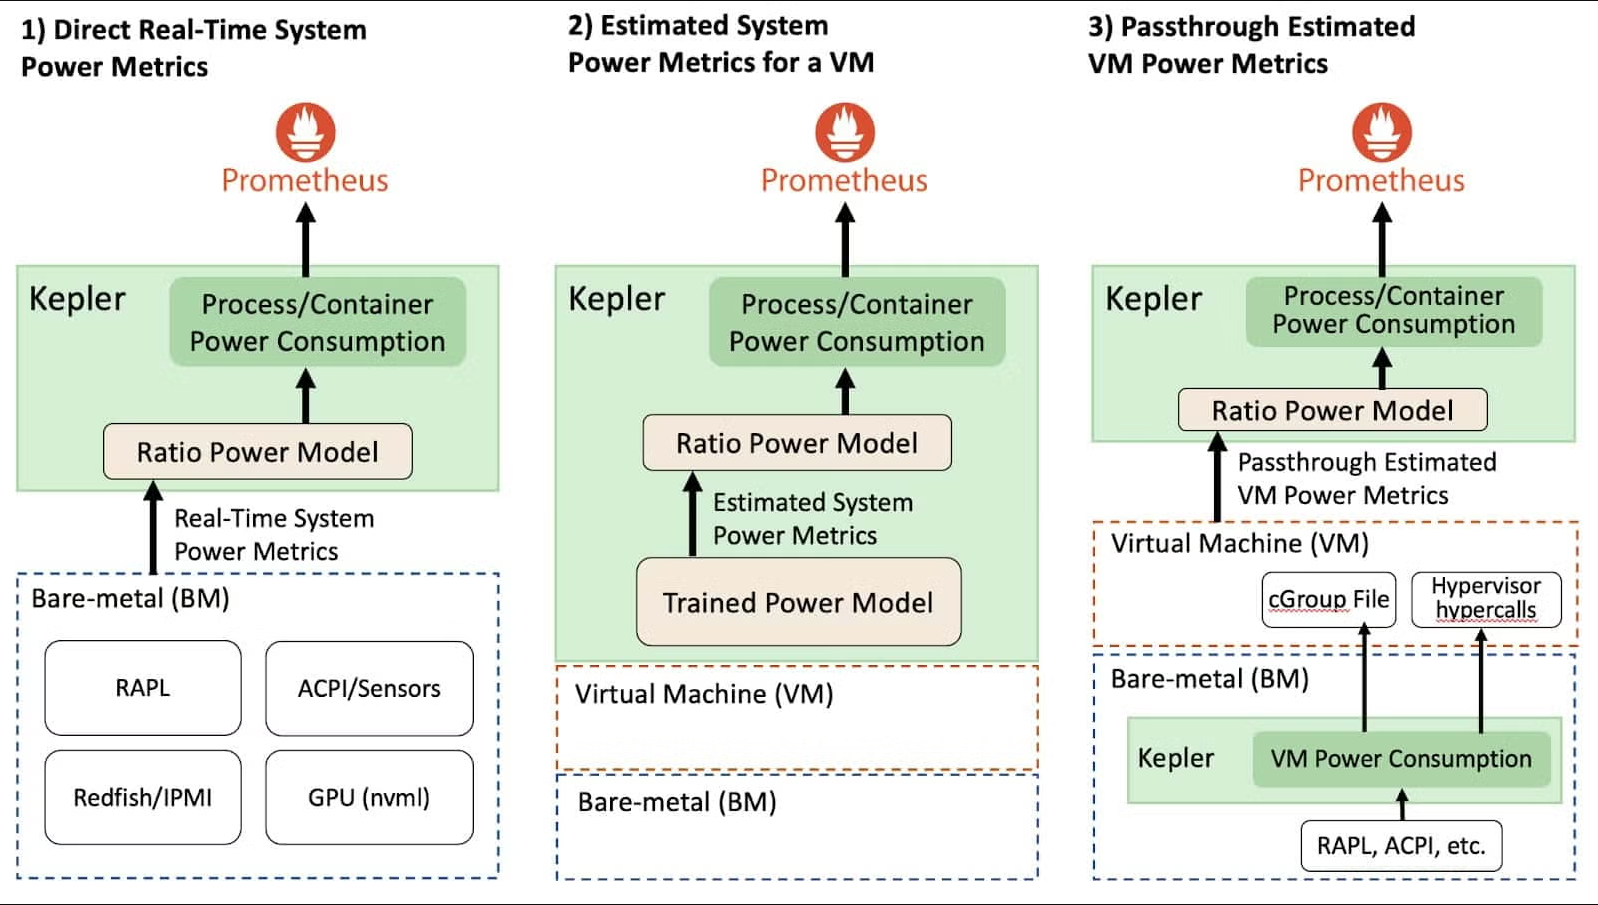
\includegraphics[width=0.85\textwidth]{figures/KeplerArchitecture.jpg}
    \caption{Architettura di Kepler per la raccolta dei consumi energetici 
    in ambienti bare-metal e virtuali. In ambienti bare-metal, Kepler 
    accede direttamente ai contatori hardware tramite RAPL, ottenendo 
    misurazioni real-time senza necessità di modelli predittivi. }
    \label{fig:kepler-arch}
\end{figure}

Come illustrato in Figura~\ref{fig:kepler-arch}, il comportamento di
Kepler varia in base all'ambiente di esecuzione. In ambienti bare-metal,
Kepler accede direttamente ai contatori RAPL, ottenendo misurazioni
energetiche real-time senza ricorrere a modelli predittivi
pre-addestrati. In ambienti virtualizzati, invece, l'assenza di accesso
diretto all'hardware richiede l'uso di modelli di regressione,
introducendo le relative limitazioni di accuratezza.

Per accedere alle interfacce hardware necessarie, Kepler deve essere 
eseguito con privilegi elevati sull'host: richiede accesso a 
\texttt{/sys} e \texttt{/proc} per leggere i contatori RAPL e i cgroup, 
e al socket Docker per identificare i container attivi e associarvi le 
metriche energetiche.
